\subsubsection{Heurísitca de Savings}

\subsubsubsection{Medición en base al tamaño del grafo}

Al comienzo de su ejecución, la herurística calcula el saving entre todo par de nodos, para luego recorrer cada uno de ellos para construir la solución final. Es de esperar entonces que savings presente una curva cuya pendiente incremente a medida que crece el valor de n.

\begin{figure}[H]
	\centering
	\begin{minipage}[t]{.45\textwidth}
		\centering
		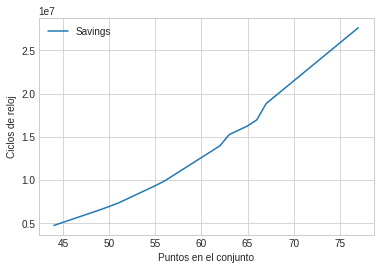
\includegraphics[scale=0.55]{exercise5/savings3}
	\end{minipage}\qquad
	\begin{minipage}[t]{.45\textwidth}
		\centering
		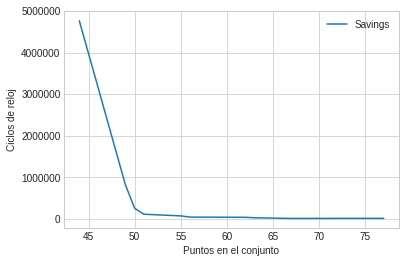
\includegraphics[scale=0.55]{exercise5/savingsAcotado}
	\end{minipage}
\end{figure}

El gráfico cumple con lo esperado y presenta una curva consistente con la creciente cantidad de puntos y la complejidad $\mathcal{O}(n^{3})$ de la heurística. Esto se puede comprobar fácilmente al visualizar el gráfico del lado derecho, que muestra la performance de savings acotada por la complejidad temporal. Al ver que el gráfico converge, podemos concluir que la heurística respeta la complejidad temporal planteada.


\subsubsubsection{Medición en base a distribución del grafo}

\begin{figure}[H]
	\centering
	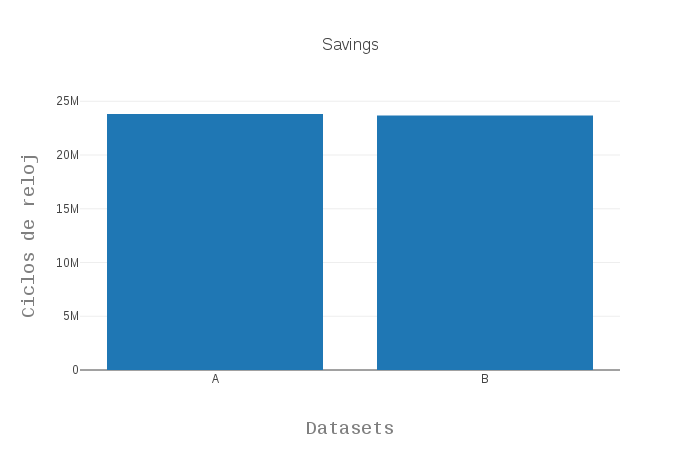
\includegraphics[scale=0.4]{exercise5/savingsType.png}
\end{figure}